% Gabarit pandoc des corrigés publiés (brut et guidé). Contenu sans marque ni nom de site.
% Compilation : lualatex (latexmk -lualatex).
% Le Markdown reste la source unique : ne pas éditer ce fichier .tex à la main.
\documentclass[11pt,a4paper]{article}

% --- Moteur, polices (Latin Modern) et langue ---------------------------------
\usepackage{iftex}
\ifLuaTeX\else\errmessage{Ce document se compile avec lualatex}\fi
\usepackage{amsmath,amssymb,mathtools}
\usepackage{fontspec}
% mathrm=sym : \mathrm prend ses glyphes dans la police mathématique (ℓ, μ, Ω), comme KaTeX.
\usepackage[math-style=TeX,bold-style=TeX,mathrm=sym]{unicode-math}
% Repli pour les glyphes absents de Latin Modern (indices et exposants Unicode,
% flèches, filets des schémas en texte, symboles) : DejaVu, puis Latin Modern Math
% (ℓ, lettres mathématiques Unicode des légendes).
\directlua{
  luaotfload.add_fallback("repliTexte", {"DejaVuSerif:mode=harf;", "DejaVuSans:mode=harf;", "file:latinmodern-math.otf:mode=harf;"})
  luaotfload.add_fallback("repliMono", {"DejaVuSansMono:mode=harf;", "DejaVuSans:mode=harf;", "file:latinmodern-math.otf:mode=harf;"})
}
\setmainfont{Latin Modern Roman}[RawFeature={fallback=repliTexte}]
\setsansfont{Latin Modern Sans}[RawFeature={fallback=repliTexte}]
\setmonofont{Latin Modern Mono}[RawFeature={fallback=repliMono}]
\setmathfont{Latin Modern Math}
\usepackage[french]{babel}
\frenchsetup{SmallCapsFigTabCaptions=false}

% --- Mise en page --------------------------------------------------------------
\usepackage[a4paper,margin=2.2cm,headheight=14pt,footskip=1.2cm]{geometry}
\usepackage{microtype}
\setlength{\emergencystretch}{4em}
\tolerance=1500
\setlength{\parindent}{0pt}
\setlength{\parskip}{0.55\baselineskip plus 2pt minus 1pt}
\usepackage{xcolor}
% Gris nommés : babel-french rend « ! » actif dans le document.
\definecolor{gris2}{gray}{0.98}
\definecolor{gris3}{gray}{0.97}
\definecolor{gris5}{gray}{0.95}
\definecolor{gris35}{gray}{0.65}
\definecolor{gris40}{gray}{0.60}
\definecolor{gris45}{gray}{0.55}
\definecolor{gris50}{gray}{0.50}
\definecolor{gris55}{gray}{0.45}
\definecolor{gris60}{gray}{0.40}
\definecolor{gris65}{gray}{0.35}
\definecolor{gris70}{gray}{0.30}
\definecolor{gris80}{gray}{0.20}
\definecolor{gris85}{gray}{0.15}
\usepackage{graphicx}
\usepackage{float}
\usepackage{caption}
\captionsetup{font=small,labelformat=empty,justification=centering}
\usepackage{booktabs,longtable,array,multirow,calc}
\usepackage{siunitx}
\sisetup{locale=FR}
\usepackage[version=4]{mhchem}
\usepackage{listings}
\usepackage{fancyhdr}
\usepackage{lastpage}
\usepackage[most]{tcolorbox}
\usepackage{enumitem}
\setlist{nosep,leftmargin=*,topsep=2pt}
\usepackage[hidelinks,unicode]{hyperref}
\usepackage{bookmark}
\hypersetup{pdftitle={CCINP MP — Mathématiques 2 2026},pdfauthor={Rédigé par IA},pdfcreator={LaTeX},pdfsubject={Corrigé brut}}
\usepackage{xurl}

% --- Pandoc : listes, tableaux, figures ----------------------------------------
\providecommand{\passthrough}[1]{#1}
\providecommand{\tightlist}{\setlength{\itemsep}{0pt}\setlength{\parskip}{0pt}}

\makeatletter
\def\maxwidth{\ifdim\Gin@nat@width>\linewidth\linewidth\else\Gin@nat@width\fi}
\def\maxheight{\ifdim\Gin@nat@height>0.55\textheight 0.55\textheight\else\Gin@nat@height\fi}
\makeatother
\setkeys{Gin}{width=\maxwidth,height=\maxheight,keepaspectratio}
\setcounter{secnumdepth}{-\maxdimen}
\providecommand{\pandocbounded}[1]{#1}

% --- Code (listings) -----------------------------------------------------------
\lstset{
  basicstyle=\ttfamily\small,
  columns=fullflexible,
  keepspaces=true,
  breaklines=true,
  breakatwhitespace=false,
  postbreak=\mbox{\textcolor{gris50}{$\hookrightarrow$}\space},
  frame=single,
  rulecolor=\color{gris35},
  framesep=4pt,
  xleftmargin=5pt,xrightmargin=5pt,
  backgroundcolor=\color{gris3},
  keywordstyle=\bfseries,
  commentstyle=\color{gris65},
  stringstyle=\color{gris80},
  showstringspaces=false,
  tabsize=4,
  extendedchars=true,
  aboveskip=6pt,belowskip=6pt,
}

% --- Macros des corrigés (KaTeX ↔ LaTeX) ---------------------------------------
% Les corrigés sont écrits pour KaTeX : on définit ici ce que KaTeX connaît et
% que LaTeX n'a pas, sans jamais retoucher le Markdown.
\providecommand{\R}{\mathbb{R}}
\providecommand{\N}{\mathbb{N}}
\providecommand{\Z}{\mathbb{Z}}
\providecommand{\Q}{\mathbb{Q}}
\providecommand{\C}{\mathbb{C}}
\providecommand{\dd}{\mathrm{d}}
\providecommand{\llbracket}{\lBrack}
\providecommand{\rrbracket}{\rBrack}
\providecommand{\lBrace}{\lbrace}
\providecommand{\rBrace}{\rbrace}
\providecommand{\Box}{\square}
\providecommand{\Diamond}{\lozenge}
\providecommand{\varnothing}{\emptyset}
\providecommand{\argmax}{\operatorname*{arg\,max}}
\providecommand{\argmin}{\operatorname*{arg\,min}}
\renewcommand{\leq}{\leqslant}
\renewcommand{\geq}{\geqslant}

% Équation hors texte : réduite à la largeur de la ligne si elle déborde.
\newsavebox{\boiteequation}
\newcommand{\equationajustee}[1]{%
  \sbox{\boiteequation}{$\displaystyle #1$}%
  \ifdim\wd\boiteequation>\linewidth
    \[\resizebox{\linewidth}{!}{\usebox{\boiteequation}}\]%
  \else
    \[#1\]%
  \fi}

% --- Encadrés pédagogiques (sobres, lisibles en noir et blanc) -----------------
\tcbset{
  encadre/.style={
    enhanced,breakable,sharp corners,
    colback=white,colframe=gris55,
    boxrule=0.4pt,leftrule=2.2pt,
    left=6pt,right=6pt,top=3pt,bottom=3pt,
    before skip=6pt,after skip=6pt,
    fonttitle=\bfseries\small,coltitle=black,
    attach title to upper,after title={\quad},
    parbox=false,
  }
}
\newtcolorbox{indication}[1]{encadre,colframe=gris45,colback=gris2,title={Indication~#1}}
\newtcolorbox{methode}{encadre,colframe=gris70,title={Méthode}}
\newtcolorbox{piege}{encadre,colframe=gris85,boxrule=0.8pt,leftrule=2.2pt,title={Piège}}
\newtcolorbox{jury}{encadre,colframe=gris60,colback=gris5,title={Jury}}
\newtcolorbox{encadrenote}{encadre,colframe=gris40}

% --- Titres de section ---------------------------------------------------------
\usepackage{titlesec}
\titleformat{\section}{\Large\bfseries}{}{0pt}{}
\titleformat{\subsection}{\large\bfseries}{}{0pt}{}
\titleformat{\subsubsection}{\normalsize\bfseries}{}{0pt}{}
\titlespacing*{\section}{0pt}{14pt plus 4pt minus 2pt}{6pt}
\titlespacing*{\subsection}{0pt}{10pt plus 3pt minus 2pt}{4pt}
\titlespacing*{\subsubsection}{0pt}{8pt plus 2pt minus 2pt}{2pt}

% --- En-tête et pied de page ---------------------------------------------------
\pagestyle{fancy}
\fancyhf{}
\fancyhead[L]{\small\textsc{Corrigé brut} · CCINP MP}
\fancyhead[R]{\small Maths 2 2026}
\fancyfoot[L]{\footnotesize Corrigé rédigé par IA, non officiel}
\fancyfoot[R]{\footnotesize \thepage\,/\,\pageref*{LastPage}}
\renewcommand{\headrulewidth}{0.4pt}
\renewcommand{\footrulewidth}{0pt}
\fancypagestyle{plain}{\fancyhf{}\fancyfoot[R]{\footnotesize \thepage\,/\,\pageref*{LastPage}}\fancyfoot[L]{\footnotesize Corrigé rédigé par IA, non officiel}\renewcommand{\headrulewidth}{0pt}}

\begin{document}
\thispagestyle{plain}
\begin{center}
  {\small\scshape Corrigé brut}\par\smallskip
  {\LARGE\bfseries CCINP MP — Mathématiques 2 2026\par}\medskip
  {\large CCINP · MP · Maths 2 · 2026\par}
\end{center}
\vspace{2pt}\hrule\vspace{8pt}

\emph{Corrigé rédigé par IA, non officiel. Signalez toute erreur.}

Épreuve MP3M2, durée 4 heures, calculatrices interdites. Deux exercices et un problème indépendants, 20 questions.

\begin{center}\rule{0.5\linewidth}{0.5pt}\end{center}

\hypertarget{exercice-1}{%
\section{Exercice 1}\label{exercice-1}}

Ici \(a,b\in\mathbb R\) avec \(a\neq 0\), et \(I=I_3\). La matrice \(J\in\mathcal M_3(\mathbb R)\) a tous ses coefficients égaux à \(1\), et \(A=aJ+bI\).

\hypertarget{q1}{%
\subsection{Q1}\label{q1}}

Les trois colonnes de \(J\) sont égales à \(u={}^t(1,1,1)\neq0\). Donc \(\operatorname{Im}J=\operatorname{Vect}(u)\) et \(\boxed{\operatorname{rg}J=1}\).

Pour tous \(i,j\), on a \((J^2)_{ij}=\sum_{k=1}^3 1\cdot1=3\), donc \(J^2=3J\).

Le polynôme \(X(X-3)\) annule donc \(J\). Il est scindé sur \(\mathbb R\) à racines simples : \(J\) est diagonalisable dans \(\mathcal M_3(\mathbb R)\), et \(\operatorname{Sp}(J)\subset\{0,3\}\).

\begin{itemize}
\tightlist
\item
  \(\ker J=\{x\in\mathbb R^3,\ x_1+x_2+x_3=0\}\) est de dimension \(3-\operatorname{rg}J=2\) (théorème du rang). Donc \(0\) est valeur propre et \(\dim E_0(J)=2\).
\item
  \(Ju=3u\) avec \(u\neq0\) : \(3\) est valeur propre. Comme \(J\) est diagonalisable, \(\dim E_0+\dim E_3=3\), d'où \(E_3(J)=\operatorname{Vect}(u)\).
\end{itemize}

\equationajustee{\boxed{J \text{ est diagonalisable, semblable \text{à} } \operatorname{diag}(3,0,0)}}

\hypertarget{q2}{%
\subsection{Q2}\label{q2}}

D'après Q1, il existe \(Q\in GL_3(\mathbb R)\) telle que \(Q^{-1}JQ=D=\operatorname{diag}(3,0,0)\). Alors
\equationajustee{Q^{-1}AQ=aQ^{-1}JQ+bI=aD+bI.}
\equationajustee{\boxed{A \text{ est semblable \text{à} } \operatorname{diag}(3a+b,\ b,\ b)}}
On a \(E_{3a+b}(A)=\operatorname{Vect}({}^t(1,1,1))\) et \(E_b(A)=\{x_1+x_2+x_3=0\}\). Comme \(a\neq0\), \(b\neq 3a+b\).

\hypertarget{q3}{%
\subsection{Q3}\label{q3}}

D'après Q2, \(A\) est diagonalisable. Par le théorème de caractérisation des matrices diagonalisables, son polynôme minimal \(\pi_A\) est donc scindé à racines simples.

Ses racines sont exactement les valeurs propres de \(A\) (toute valeur propre est racine de tout polynôme annulateur, et \(\pi_A\) divise \(\chi_A\)). Ce sont \(b\) et \(3a+b\), distinctes car \(a\neq0\).

Comme \(\pi_A\) est unitaire :
\equationajustee{\boxed{\pi_A=(X-b)(X-3a-b)}}

\hypertarget{q4}{%
\subsection{Q4}\label{q4}}

On pose \(\lambda=3a+b\), de sorte que \(\lambda-b=3a\neq0\).

\textbf{a)} Soit \(n\in\mathbb N\). Comme \(\deg\pi_A=2\), la division euclidienne s'écrit \(X^n=\pi_A Q_n+R_n\), avec \(R_n=\alpha_nX+\beta_n\).

En évaluant en les racines \(b\) et \(\lambda\) de \(\pi_A\) :
\equationajustee{\begin{aligned}
b^n&=\alpha_nb+\beta_n,\\
\lambda^n&=\alpha_n\lambda+\beta_n.
\end{aligned}}
Par différence, puis en reportant :
\equationajustee{\begin{aligned}
\alpha_n&=\frac{\lambda^n-b^n}{\lambda-b}=\frac{\lambda^n-b^n}{3a},\\
\beta_n&=b^n-\alpha_nb=\frac{\lambda b^n-b\lambda^n}{3a}.
\end{aligned}}
Comme \(\pi_A(A)=0\), on a \(A^n=\pi_A(A)Q_n(A)+R_n(A)=R_n(A)\) :
\equationajustee{\boxed{\forall n\in\mathbb N,\ A^n=\frac{\lambda^n-b^n}{3a}\,A+\frac{\lambda b^n-b\lambda^n}{3a}\,I,\ \text{avec } \lambda=3a+b}}
Contrôle : \(n=0\) donne \(I\), \(n=1\) donne \(A\).

\textbf{b)} Par récurrence, \(J^k=3^{k-1}J\) pour tout \(k\ge1\). C'est vrai pour \(k=1\), et si \(J^k=3^{k-1}J\), alors \(J^{k+1}=3^{k-1}J^2=3^kJ\).
\equationajustee{\boxed{\forall k\ge1,\quad J^k=3^{k-1}J}}
Les matrices \(aJ\) et \(bI\) commutent, donc la formule du binôme s'applique. La formule de \(J^k\) ne vaut que pour \(k\ge1\) : on isole le terme \(k=0\), pour lequel \(J^0=I\).
\equationajustee{\begin{aligned}
A^n&=\sum_{k=0}^n\binom nk a^kb^{n-k}J^k\\
&=b^nI+\frac13\Big(\sum_{k=1}^n\binom nk(3a)^kb^{n-k}\Big)J\\
&=b^nI+\frac{(3a+b)^n-b^n}{3}\,J.
\end{aligned}}
\equationajustee{\boxed{\forall n\in\mathbb N,\quad A^n=b^n\,I+\frac{(3a+b)^n-b^n}{3}\,J}}
Cohérence avec a), en remplaçant \(A\) par \(aJ+bI\) :
\equationajustee{\begin{aligned}
\alpha_nA+\beta_nI&=\alpha_na\,J+(\alpha_nb+\beta_n)I\\
&=\frac{\lambda^n-b^n}{3}J+b^nI.
\end{aligned}}

\begin{center}\rule{0.5\linewidth}{0.5pt}\end{center}

\hypertarget{exercice-2}{%
\section{Exercice 2}\label{exercice-2}}

Ici \(n\in\mathbb N^*\) et \(P=a_0+a_1X+\dots+a_{n-1}X^{n-1}\in\mathbb R[X]\). Pour \(k\in[\![0,n-1]\!]\), \(\omega_k=\mathrm e^{2ik\pi/n}\). On veut montrer \((*)\) : \(P(\omega_1)\cdots P(\omega_{n-1})\in\mathbb R\).

\hypertarget{q5}{%
\subsection{Q5}\label{q5}}

\(j\neq1\) et \(j^3=1\), donc \(1+j+j^2=\dfrac{j^3-1}{j-1}\) :
\equationajustee{\boxed{1+j+j^2=0}}
On prend \(n=3\) et \(P=1+2X+3X^2\) : degré \(2\), coefficients réels, non nuls et deux à deux distincts. Ici \(\omega_1=j\) et \(\omega_2=j^2\).

Avec \(j^2=-1-j\) et \(j^4=j\) :
\equationajustee{\begin{aligned}
P(j)&=1+2j+3j^2\\
&=-2-j,\\
P(j^2)&=1+2j^2+3j^4\\
&=1+3j+2j^2\\
&=-1+j.
\end{aligned}}
Donc :
\equationajustee{\begin{aligned}
P(j)P(j^2)&=(-2-j)(-1+j)\\
&=2-j-j^2\\
&=3.
\end{aligned}}
\equationajustee{\boxed{P(\omega_1)P(\omega_2)=3\in\mathbb R}}
Cela vérifie \((*)\). On note d'ailleurs que \(j^2=\overline j\), et que le produit vaut \(|P(j)|^2\).

\hypertarget{q6}{%
\subsection{Q6}\label{q6}}

\(J\) est définie par \(J_{i,i+1}=1\) pour \(1\le i\le n-1\) et \(J_{n,1}=1\), les autres coefficients étant nuls. On note \(\chi_J=\det(XI_n-J)\).

Si \(n=1\), \(J=(1)\) et \(\chi_J=X-1\).

Si \(n\ge2\), soit \(M=XI_n-J\). Sa première colonne n'a que deux coefficients non nuls : \(M_{1,1}=X\) et \(M_{n,1}=-1\). En développant selon cette colonne :
\equationajustee{\chi_J=X\,\Delta_{1,1}+(-1)\cdot(-1)^{n+1}\,\Delta_{n,1},}
où \(\Delta_{i,1}\) est le mineur obtenu en supprimant la ligne \(i\) et la colonne \(1\).

\begin{itemize}
\tightlist
\item
  \(\Delta_{1,1}\) : la sous-matrice est triangulaire supérieure, de diagonale \(X\) (et de sur-diagonale \(-1\)). Donc \(\Delta_{1,1}=X^{n-1}\).
\item
  \(\Delta_{n,1}\) : on garde les lignes \(1\) à \(n-1\) et les colonnes \(2\) à \(n\).
  La sous-matrice est triangulaire inférieure, de diagonale \(-1\) (les \(-1\) de \(M\) en position \((i,i+1)\)) et de sous-diagonale \(X\). Donc \(\Delta_{n,1}=(-1)^{n-1}\).
\end{itemize}

D'où :
\equationajustee{\begin{aligned}
\chi_J&=X^n+(-1)^{n+2}(-1)^{n-1}\\
&=X^n+(-1)^{2n+1}.
\end{aligned}}
\equationajustee{\boxed{\chi_J=X^n-1}}
Contrôle : pour \(n=3\), la règle de Sarrus donne \(X^3-1\).

\hypertarget{q7}{%
\subsection{Q7}\label{q7}}

On a \(J_{i,j}=1\) si \(j\equiv i+1\ [n]\), et \(0\) sinon.

Par récurrence sur \(k\) : \((J^k)_{i,j}=1\) si \(j\equiv i+k\ [n]\), \(0\) sinon.

En effet, dans \((J^{k+1})_{i,j}=\sum_\ell (J^k)_{i,\ell}J_{\ell,j}\), seul le terme \(\ell\equiv i+k\) est non nul. Il vaut \(1\) si et seulement si \(j\equiv i+k+1\).

Pour \(i,j\) fixés, un seul \(k\in[\![0,n-1]\!]\) vérifie \(j\equiv i+k\ [n]\), à savoir \(k=(j-i)\bmod n\). Donc :
\equationajustee{\begin{aligned}
P(J)_{i,j}&=\sum_{k=0}^{n-1}a_k(J^k)_{i,j}\\
&=a_{(j-i)\bmod n}.
\end{aligned}}
La première ligne est \((a_0,a_1,\dots,a_{n-1})\). Chaque ligne se déduit de la précédente par un décalage circulaire d'une case vers la droite : c'est la description de \(A\).
\equationajustee{\boxed{A=P(J)}}

\hypertarget{q8}{%
\subsection{Q8}\label{q8}}

D'après Q7, \((J^n)_{i,j}=1\) si et seulement si \(j\equiv i\ [n]\), donc \(J^n=I_n\).

Le polynôme \(X^n-1=\prod_{k=0}^{n-1}(X-\omega_k)\) annule donc \(J\). Il est scindé sur \(\mathbb C\) à racines simples, car les \(\omega_k\) sont deux à deux distincts. Donc \(J\) est diagonalisable dans \(\mathcal M_n(\mathbb C)\).

D'après Q6, ses valeurs propres sont les \(n\) racines de \(\chi_J=X^n-1\), toutes simples. Il existe donc \(Q\in GL_n(\mathbb C)\) telle que
\equationajustee{\boxed{Q^{-1}JQ=\Delta=\operatorname{diag}(\omega_0,\omega_1,\dots,\omega_{n-1})}}
On peut prendre pour colonnes de \(Q\) les vecteurs \(V_k={}^t(1,\omega_k,\omega_k^2,\dots,\omega_k^{n-1})\), qui vérifient \(JV_k=\omega_kV_k\).

Comme \(J^m=Q\Delta^mQ^{-1}\) pour tout \(m\), par linéarité \(A=P(J)=Q\,P(\Delta)\,Q^{-1}\), et \(P(\Delta)\) est diagonale :
\equationajustee{\boxed{Q^{-1}AQ=\operatorname{diag}\big(P(\omega_0),P(\omega_1),\dots,P(\omega_{n-1})\big)}}
Les \(P(\omega_k)\) ne sont pas forcément distincts : pour \(n=4\) et \(P=X+X^3\), \(P(i)=P(-i)=0\).

\hypertarget{q9}{%
\subsection{Q9}\label{q9}}

Si \(n=1\), le produit est vide et vaut \(1\). Supposons \(n\ge2\). D'après Q8 :
\equationajustee{\begin{aligned}
\det A&=\prod_{k=0}^{n-1}P(\omega_k)\\
&=P(1)\prod_{k=1}^{n-1}P(\omega_k).
\end{aligned}}
Or \(\det A\in\mathbb R\) car \(A\) est réelle, et \(P(1)=a_0+\dots+a_{n-1}\in\mathbb R\).

\begin{itemize}
\tightlist
\item
  Si \(P(1)\neq0\) : \(\prod_{k=1}^{n-1}P(\omega_k)=\dfrac{\det A}{P(1)}\in\mathbb R\).
\item
  Cas général, y compris \(P(1)=0\). Pour \(x\in\mathbb R\), le polynôme \(P+x\) est à coefficients réels et sa matrice circulante est \(A+xI_n\). Q8 appliquée à \(P+x\) donne \(\det(A+xI_n)=\prod_{k=0}^{n-1}(P(\omega_k)+x)\).
\item
  La fonction \(R:x\mapsto\prod_{k=1}^{n-1}(P(\omega_k)+x)\) est polynomiale, donc continue de \(\mathbb R\) dans \(\mathbb C\). Pour \(x\neq-P(1)\), \(R(x)=\dfrac{\det(A+xI_n)}{P(1)+x}\) est réel d'après le premier point.
\item
  Comme \(\mathbb R\) est fermé dans \(\mathbb C\), \(R(0)=\lim_{x\to0,\,x\neq-P(1)}R(x)\in\mathbb R\).
\end{itemize}

\equationajustee{\boxed{P(\omega_1)P(\omega_2)\cdots P(\omega_{n-1})\in\mathbb R}}

\emph{Remarque (vérification directe).} \(P\) étant réel, \(\overline{P(\omega_k)}=P(\overline{\omega_k})=P(\omega_{n-k})\). Et \(k\mapsto n-k\) est une bijection de \([\![1,n-1]\!]\) : le produit est égal à son conjugué.

\begin{figure}[H]
\centering
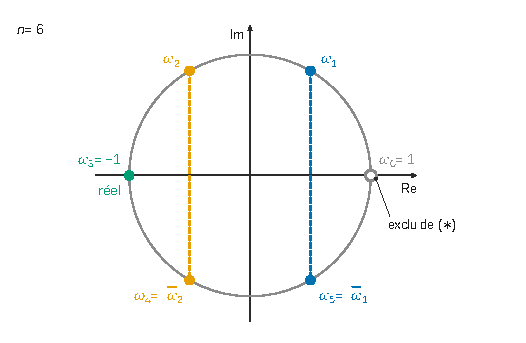
\includegraphics{figures/q9-racines-conjuguees.pdf}
\caption*{Figure 1 --- Cas n = 6 : ω\_0 = 1 est exclu du produit (∗), les autres
racines s'apparient en conjugués ω\_5 = ω̄\_1, ω\_4 = ω̄\_2, et ω\_3 = −1
est réel}
\end{figure}

\begin{center}\rule{0.5\linewidth}{0.5pt}\end{center}

\hypertarget{probluxe8me}{%
\section{Problème}\label{probluxe8me}}

\hypertarget{q10-question-de-cours}{%
\subsection{Q10 --- Question de cours}\label{q10-question-de-cours}}

On n'utilise que la définition de \(p_F(x)\) donnée par l'énoncé (unique vecteur de \(F\) tel que \(x-p_F(x)\in F^\perp\)) ; \(E\) n'est pas supposé de dimension finie.

\textbf{a)} Soit \(x\in E\) et \(y=\sum_{i=0}^n\langle x\mid e_i\rangle e_i\), qui appartient à \(F\). Pour \(j\in[\![0,n]\!]\), par linéarité à gauche et orthonormalité :
\equationajustee{\begin{aligned}
\langle x-y\mid e_j\rangle&=\langle x\mid e_j\rangle-\sum_{i=0}^n\langle x\mid e_i\rangle\langle e_i\mid e_j\rangle\\
&=\langle x\mid e_j\rangle-\langle x\mid e_j\rangle\\
&=0.
\end{aligned}}
Donc \(x-y\) est orthogonal à chaque \(e_j\). Par linéarité, il est orthogonal à tout vecteur de \(F=\operatorname{Vect}(e_0,\dots,e_n)\) : \(x-y\in F^\perp\).

Par unicité du vecteur de \(F\) ayant cette propriété :
\equationajustee{\boxed{p_F(x)=\sum_{i=0}^n\langle x\mid e_i\rangle\,e_i}}

\textbf{b)} Posons \(p=p_F(x)\). Comme \(p\in F\) et \(x-p\in F^\perp\), on a \(\langle p\mid x-p\rangle=0\). Le théorème de Pythagore donne :
\equationajustee{\begin{aligned}
\|x\|^2&=\|p\|^2+\|x-p\|^2\\
&\ge\|p\|^2.
\end{aligned}}
\equationajustee{\boxed{\|p_F(x)\|^2\le\|x\|^2}}

\begin{figure}[H]
\centering
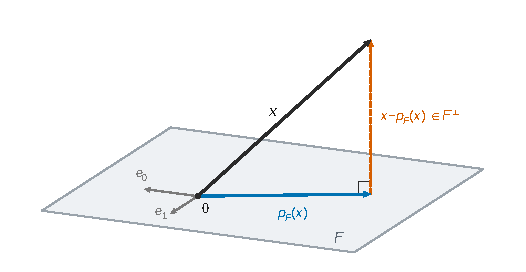
\includegraphics{figures/q10-projection-orthogonale.pdf}
\caption*{Figure 2 --- Projeté orthogonal : p\_F(x) ∈ F et x − p\_F(x) ∈ F⊥ sont
les côtés de l'angle droit d'un triangle rectangle d'hypoténuse x}
\end{figure}

La famille \((e_i)\) étant orthonormale, Pythagore donne aussi \(\|p\|^2=\sum_{i=0}^n\langle x\mid e_i\rangle^2\), d'où :
\equationajustee{\boxed{\sum_{i=0}^n\langle x\mid e_i\rangle^2\le\|x\|^2}}

\hypertarget{q11}{%
\subsection{Q11}\label{q11}}

Comme \(|a|^2=a^2\) et \(|b|^2=b^2\), l'inégalité \((|a|-|b|)^2\ge0\) s'écrit \(a^2+b^2-2|a||b|\ge0\). Avec \(|ab|=|a||b|\) :
\equationajustee{\boxed{|ab|\le\frac{a^2+b^2}{2}}}
Soient \(f,g\in E\). La fonction \(\varphi:t\mapsto f(t)g(t)\mathrm e^{-t}\) est continue sur \(I\).

Pour tout \(t\in I\), l'inégalité précédente appliquée à \(f(t)\) et \(g(t)\), multipliée par \(\mathrm e^{-t}>0\), donne :
\equationajustee{|\varphi(t)|\le\tfrac12\big(f(t)^2\mathrm e^{-t}+g(t)^2\mathrm e^{-t}\big).}
Le majorant est intégrable sur \(I\) (définition de \(E\)). Par comparaison, \textbf{\(t\mapsto f(t)g(t)\mathrm e^{-t}\) est intégrable sur \(I\).}

\hypertarget{q12}{%
\subsection{Q12}\label{q12}}

\emph{\(E\) est un espace vectoriel.} \(E\) est une partie de l'espace vectoriel \(\mathcal C(I,\mathbb R)\), qui contient la fonction nulle. Soient \(f,g\in E\) et \(\lambda\in\mathbb R\). La fonction \(f+\lambda g\) est continue, et :
\equationajustee{(f+\lambda g)^2(t)\mathrm e^{-t}=f(t)^2\mathrm e^{-t}+2\lambda f(t)g(t)\mathrm e^{-t}+\lambda^2g(t)^2\mathrm e^{-t}.}
C'est une combinaison linéaire de fonctions intégrables sur \(I\) : \(f^2\mathrm e^{-t}\) et \(g^2\mathrm e^{-t}\) par définition de \(E\), \(fg\,\mathrm e^{-t}\) par Q11.

Donc \(f+\lambda g\in E\) : \textbf{\(E\) est un sous-espace vectoriel de \(\mathcal C(I,\mathbb R)\).}

\emph{Produit scalaire.} D'après Q11, l'intégrale \(\langle f\mid g\rangle\) converge pour tous \(f,g\in E\) : l'application est bien définie sur \(E^2\).

\begin{itemize}
\tightlist
\item
  Symétrie : \(f(t)g(t)\mathrm e^{-t}=g(t)f(t)\mathrm e^{-t}\).
\item
  Linéarité à gauche : soient \(f_1,f_2,g\in E\) et \(\lambda\in\mathbb R\). Les intégrales \(\langle f_1\mid g\rangle\) et \(\langle f_2\mid g\rangle\) convergent (Q11). La linéarité de l'intégrale sur les intégrales convergentes donne \(\langle f_1+\lambda f_2\mid g\rangle=\langle f_1\mid g\rangle+\lambda\langle f_2\mid g\rangle\). Par symétrie, l'application est bilinéaire.
\item
  Positivité : \(\langle f\mid f\rangle=\int_0^{+\infty}f(t)^2\mathrm e^{-t}\,\mathrm dt\ge0\).
\item
  Caractère défini : si \(\langle f\mid f\rangle=0\), la fonction \(t\mapsto f(t)^2\mathrm e^{-t}\) est \textbf{continue}, positive, intégrable et d'intégrale nulle sur \(I\). Elle est donc nulle sur \(I\). Comme \(\mathrm e^{-t}>0\), \(f=0\).
\end{itemize}

\textbf{\(\langle\ \mid\ \rangle\) est un produit scalaire sur \(E\).}

\hypertarget{q13}{%
\subsection{Q13}\label{q13}}

\emph{Inclusion \(F\subset E\).} Soit \(P\in\mathbb R_n[X]\). La fonction \(t\mapsto P(t)^2\mathrm e^{-t}\) est continue et positive sur \(I\).

Par croissances comparées, \(t^2P(t)^2\mathrm e^{-t}\to0\) quand \(t\to+\infty\), donc \(P(t)^2\mathrm e^{-t}=o(1/t^2)\).

Comme \(t\mapsto1/t^2\) est intégrable sur \([1,+\infty[\), \(P^2\mathrm e^{-t}\) l'est aussi. Elle est intégrable sur le segment \([0,1]\) par continuité. Donc \(P\in E\).

\emph{Structure.} Ainsi \(F\subset E\). De plus \(F=\mathbb R_n[X]\) est lui-même un espace vectoriel : il contient \(0\) et il est stable par combinaison linéaire.

Les lois de \(E\) restreintes à \(F\) sont celles de \(\mathbb R_n[X]\). Donc \textbf{\(F\) est un sous-espace vectoriel de \(E\).}

L'identification d'un polynôme à sa fonction sur \(I\) est injective : un polynôme qui s'annule sur l'ensemble infini \(I\) est nul. Donc \(\dim F=n+1\), et \(\langle\ \mid\ \rangle\) est un produit scalaire sur \(\mathbb R[X]\) (le même argument vaut pour tout \(\mathbb R_m[X]\)).

\hypertarget{q14}{%
\subsection{Q14}\label{q14}}

\textbf{a)} \(u:x\mapsto x^n\) et \(v:x\mapsto\mathrm e^{-x}\) sont de classe \(\mathcal C^\infty\).

Pour \(k\le n\), \(u^{(k)}(x)=\frac{n!}{(n-k)!}x^{n-k}\), et \(v^{(m)}(x)=(-1)^m\mathrm e^{-x}\). Pour \(p\le n\), la formule de Leibniz donne :
\equationajustee{\boxed{h_n^{(p)}(x)=\mathrm e^{-x}\sum_{k=0}^p(-1)^{p-k}\binom pk\frac{n!}{(n-k)!}\,x^{n-k}}}
Si \(p<n\), chaque exposant vérifie \(n-k\ge n-p\ge1\). Chaque terme s'annule donc en \(0\) :
\equationajustee{\boxed{p<n\implies h_n^{(p)}(0)=0}}

\textbf{b)} Avec \(p=n\) :
\equationajustee{\begin{aligned}
L_n(x)&=\frac{\mathrm e^x}{n!}h_n^{(n)}(x)\\
&=\sum_{k=0}^n(-1)^{n-k}\binom nk\frac{x^{n-k}}{(n-k)!}.
\end{aligned}}
Le changement d'indice \(m=n-k\) donne :
\equationajustee{\boxed{L_n=\sum_{m=0}^n(-1)^m\binom nm\frac{X^m}{m!}\in\mathbb R[X]}}
\equationajustee{\boxed{\deg L_n=n,\ \text{de coefficient dominant } \frac{(-1)^n}{n!}}}
En effet, le coefficient de \(X^n\) est \(\frac{(-1)^n}{n!}\neq0\). Par exemple \(L_0=1\), \(L_1=1-X\) et \(L_2=1-2X+\frac{X^2}2\).

\hypertarget{q15}{%
\subsection{Q15}\label{q15}}

\emph{Remarque sur l'énoncé.} Le crochet de Q12 porte le poids \(\mathrm e^{-t}\). Lu ainsi, \(\langle g\mid h_n^{(n)}\rangle=\int_0^{+\infty}g\,h_n^{(n)}\mathrm e^{-t}\) ne s'exprime pas à l'aide de \(\int_0^{+\infty}g^{(n)}h_n\).

Par exemple, pour \(n=1\) et \(g=1\), le premier vaut \(\int_0^{+\infty}(1-t)\mathrm e^{-2t}\mathrm dt=\frac14\), le second \(0\).

On remplace donc la première demande par : exprimer \(\int_0^{+\infty}g(t)h_n^{(n)}(t)\,\mathrm dt\) (intégrale sans poids) en fonction de \(\int_0^{+\infty}g^{(n)}(t)h_n(t)\,\mathrm dt\). Cette intégrale vaut \(n!\,\langle g\mid L_n\rangle\), puisque \(h_n^{(n)}(t)=n!\,L_n(t)\mathrm e^{-t}\).

Soit \(g\in\mathbb R[X]\). D'après Q14.a, toutes les fonctions \(g^{(p)}h_n^{(q)}\) sont de la forme \(t\mapsto R(t)\mathrm e^{-t}\) avec \(R\) polynomiale. Elles sont donc intégrables sur \(I\) (comme en Q13).

Montrons par récurrence sur \(p\in[\![0,n]\!]\) :
\equationajustee{\int_0^{+\infty}g\,h_n^{(n)}=(-1)^p\int_0^{+\infty}g^{(p)}h_n^{(n-p)}.}
C'est clair pour \(p=0\). Supposons-le vrai pour un \(p\le n-1\). Une intégration par parties sur \([0,A]\) donne :
\equationajustee{\int_0^Ag^{(p)}h_n^{(n-p)}=\Big[g^{(p)}h_n^{(n-p-1)}\Big]_0^A-\int_0^Ag^{(p+1)}h_n^{(n-p-1)}.}
En \(0\), \(h_n^{(n-p-1)}(0)=0\) par Q14.a car \(n-p-1<n\). En \(A\), le crochet est de la forme \(R(A)\mathrm e^{-A}\), qui tend vers \(0\).

Les intégrales convergeant, on fait \(A\to+\infty\) :
\equationajustee{\int_0^{+\infty}g^{(p)}h_n^{(n-p)}=-\int_0^{+\infty}g^{(p+1)}h_n^{(n-p-1)}.}
D'où le rang \(p+1\). Pour \(p=n\) :
\equationajustee{\boxed{\int_0^{+\infty}g(t)h_n^{(n)}(t)\,\mathrm dt=(-1)^n\int_0^{+\infty}g^{(n)}(t)h_n(t)\,\mathrm dt}}
Avec \(h_n^{(n)}=n!\,L_n\mathrm e^{-t}\) et \(h_n(t)=t^n\mathrm e^{-t}\) :
\equationajustee{\boxed{\langle g\mid L_n\rangle=\frac{(-1)^n}{n!}\int_0^{+\infty}g^{(n)}(t)\,t^n\mathrm e^{-t}\,\mathrm dt}}

\hypertarget{q16}{%
\subsection{Q16}\label{q16}}

Soient \(i<j\). \(L_i\) est un polynôme de degré \(i<j\), donc \(L_i^{(j)}=0\). Q15 appliquée à \(g=L_i\) avec l'indice \(j\) donne une intégrale convergente, d'intégrande nul :
\equationajustee{\langle L_i\mid L_j\rangle=\frac{(-1)^j}{j!}\int_0^{+\infty}L_i^{(j)}(t)\,t^j\mathrm e^{-t}\,\mathrm dt.}
\equationajustee{\boxed{\langle L_i\mid L_j\rangle=0}}

\hypertarget{q17}{%
\subsection{Q17}\label{q17}}

Soit \(I_n=\int_0^{+\infty}t^n\mathrm e^{-t}\,\mathrm dt\).

\emph{Existence.} \(t\mapsto t^n\mathrm e^{-t}\) est continue et positive sur \(I\). Par croissances comparées, \(t^{n+2}\mathrm e^{-t}\to0\) en \(+\infty\), donc \(t^n\mathrm e^{-t}=o(1/t^2)\) : l'intégrale converge.

\emph{Calcul.} \(I_0=1\). Pour \(n\ge1\), une intégration par parties sur \([0,A]\) donne :
\equationajustee{\int_0^At^n\mathrm e^{-t}\,\mathrm dt=-A^n\mathrm e^{-A}+n\int_0^At^{n-1}\mathrm e^{-t}\,\mathrm dt.}
Comme \(A^n\mathrm e^{-A}\to0\), on obtient avec \(A\to+\infty\) la relation \(I_n=nI_{n-1}\), puis par récurrence :
\equationajustee{\boxed{\int_0^{+\infty}t^n\mathrm e^{-t}\,\mathrm dt=n!}}
\(L_n\) est de degré \(n\), de coefficient dominant \(\frac{(-1)^n}{n!}\). Donc \(L_n^{(n)}=n!\cdot\frac{(-1)^n}{n!}=(-1)^n\). Par Q15 :
\equationajustee{\begin{aligned}
\langle L_n\mid L_n\rangle&=\frac{(-1)^n}{n!}\int_0^{+\infty}(-1)^nt^n\mathrm e^{-t}\,\mathrm dt\\
&=\frac{n!}{n!}.
\end{aligned}}
\equationajustee{\boxed{\langle L_n\mid L_n\rangle=1}}

\hypertarget{q18}{%
\subsection{Q18}\label{q18}}

Les \(L_i\) (\(0\le i\le n\)) sont dans \(F=\mathbb R_n[X]\) (Q14.b). Par Q16, Q17 et symétrie, \(\langle L_i\mid L_j\rangle=\delta_{ij}\).

Une famille orthonormale est libre ; celle-ci compte \(n+1=\dim F\) vecteurs :
\equationajustee{\boxed{(L_0,L_1,\dots,L_n)\text{ est une base orthonormale de }F}}
\(F\) est un sous-espace de dimension finie de l'espace préhilbertien \(E\). Q10.a donne, pour tout \(g\in E\) :
\equationajustee{\boxed{p_F(g)=\sum_{k=0}^n\langle g\mid L_k\rangle\,L_k}}

\hypertarget{q19}{%
\subsection{Q19}\label{q19}}

Soit \(g\in E\) et \(N\in\mathbb N\). Le raisonnement de Q18, avec \(N\) au lieu de \(n\), montre que \((L_0,\dots,L_N)\) est une base orthonormale de \(\mathbb R_N[X]\).

C'est un sous-espace de dimension finie de \(E\), et Q10.b donne :
\equationajustee{\sum_{k=0}^N\langle g\mid L_k\rangle^2\le\|g\|^2.}
La série \(\sum\langle g\mid L_n\rangle^2\) est à termes positifs : ses sommes partielles sont croissantes. Elles sont majorées par \(\|g\|^2\), qui ne dépend pas de \(N\). La série converge donc, et le passage à la limite dans l'inégalité donne :
\equationajustee{\boxed{\sum_{n=0}^{+\infty}\langle g\mid L_n\rangle^2\le\|g\|^2}}
avec \(\|g\|^2=\int_0^{+\infty}g(t)^2\mathrm e^{-t}\,\mathrm dt\).

\hypertarget{q20}{%
\subsection{Q20}\label{q20}}

\emph{Remarque sur l'énoncé.} L'affirmation « pour tout \(\alpha\in\mathbb R\), \(g_\alpha\in E\) » est fausse. On montre que \(g_\alpha\in E\iff\alpha>-\frac12\), ce qui est l'hypothèse posée au début de la question.

\emph{Appartenance à \(E\).} \(g_\alpha\) est continue et \(g_\alpha(t)^2\mathrm e^{-t}=\mathrm e^{-(2\alpha+1)t}\).

Cette fonction positive est intégrable sur \([0,+\infty[\) si et seulement si \(2\alpha+1>0\) (si \(2\alpha+1\le0\), elle est minorée par \(1\)).
\equationajustee{\boxed{g_\alpha\in E\iff\alpha>-\tfrac12}}
Dans ce cas :
\equationajustee{\boxed{\|g_\alpha\|^2=\int_0^{+\infty}\mathrm e^{-(2\alpha+1)t}\,\mathrm dt=\frac1{2\alpha+1}}}

\emph{Coefficients.} Soit \(\alpha>-\frac12\) et \(\beta=\alpha+1>0\).

Pour \(m\in\mathbb N\), le changement de variable \(u=\beta t\) (bijection affine croissante de \(I\) sur \(I\)) et Q17 donnent \(\int_0^{+\infty}t^m\mathrm e^{-\beta t}\,\mathrm dt=\frac{m!}{\beta^{m+1}}\). Par linéarité (somme finie) et Q14.b :
\equationajustee{\begin{aligned}
\langle g_\alpha\mid L_n\rangle&=\int_0^{+\infty}L_n(t)\mathrm e^{-\beta t}\,\mathrm dt\\
&=\sum_{m=0}^n(-1)^m\binom nm\frac1{m!}\cdot\frac{m!}{\beta^{m+1}}\\
&=\frac1\beta\Big(1-\frac1\beta\Big)^n.
\end{aligned}}
\equationajustee{\boxed{\langle g_\alpha\mid L_n\rangle=\frac{\alpha^n}{(\alpha+1)^{n+1}}}}
On retrouverait ce résultat par la formule de Q15, qui s'étend à \(g_\alpha\) : les termes de bord sont de la forme \(R(A)\mathrm e^{-\beta A}\), qui tend vers \(0\).

\emph{Somme.} Posons \(q=\frac\alpha{\alpha+1}\). Comme \(\alpha+1>0\) :
\equationajustee{\begin{aligned}
|q|<1&\iff-(\alpha+1)<\alpha<\alpha+1\\
&\iff\alpha>-\tfrac12,
\end{aligned}}
ce qui est le cas. La série géométrique de raison \(q^2\in[0,1[\) converge, et :
\equationajustee{\begin{aligned}
\sum_{n=0}^{+\infty}\langle g_\alpha\mid L_n\rangle^2&=\frac1{(\alpha+1)^2}\cdot\frac1{1-q^2}\\
&=\frac1{(\alpha+1)^2-\alpha^2}\\
&=\frac1{2\alpha+1}.
\end{aligned}}
\equationajustee{\boxed{\sum_{n=0}^{+\infty}\langle g_\alpha\mid L_n\rangle^2=\|g_\alpha\|^2}}
L'inégalité de Bessel de Q19 est une égalité pour les fonctions \(g_\alpha\).

\textbf{FIN}

\end{document}
